% INTRODUÇÃO-------------------------------------------------------------------

\chapter{INTRODUÇÃO}
\label{chap:introducao}

Dutos de ventilação usados nos sistemas de ar-condicionado estão sujeitos a diversos tipos de danos, dentre os quais pode-se listar os entupimentos progressivos devido ao acúmulo de poeira e de pequenos animais mortos. \citeonline{carmo1999qualidade} Por normalmente ser locais de difícil acesso, apresentam dificuldades em sua manutenção, favorecendo a proliferação de bactérias e transmissão de vírus \citeonline{bortoletto2002contaminaccao}.\par
Subestações de energia elétrica, em grande parte das vezes, ficam expostas a intempéries, que causam oxidações em suportes, equipamentos e cabos. Sua inspeção oferece riscos a vida por expor o corpo humano a uma quantidade enorme de energia, apesar de existir norma rigorosa para a realização de inspeções preventivas, acidentes com vítima ainda acontecem \citeonline{santos2012inspeccao}.\par
A inspeção de reservatórios de produtos químicos requer uma minuciosa análise estrutural, uma busca por áreas oxidadas e falhas em pontos de solda, que demanda muitas horas de trabalho humano. A exposição a gases e vapores tóxicos, por menor que seja a quantidade, causam riscos a saúde do inspetor \citeonline{molina2008metodo}.\par
Os casos citados, são apenas algumas das atividades extremamente necessárias no ambiente industrial, que expõem a saúde das pessoas a riscos e que podem ser evitados através de dispositivos especializados. \par 
Robôs equipados com ferramentas adequadas para cada tarefa, que podem oferecer um sistema de navegação autônomo ou de controle remoto, podem ser usados para evitar ou minimizar os riscos a saúde dos inspetores. Como exemplo, o robô \textit{SENSABOT}, usado pela Shell, para monitorar e inspecionar a planta de óleo e gás, mostrado na \autoref{fig:sensabot}, e o robô \textit{ABB}, usado em inspeções de transformadores, sem a necessidade de drenar o óleo, visto na \autoref{fig:abb}. Contudo o uso de robôs não se restringe apenas ao ambiente industrial, no ano de 2011, robôs submarinos foram usados na localização e resgate das peças do avião da Air France 447, que caiu no Oceano Atlântico em 2009. Foram usados robôs de inspeção para verificar as condições estruturais da usina nuclear de Fukushima Daiichi no Japão, que foi afetada por um tsunami. 

\begin{figure}[H]
	\centering
	\begin{subfigure}{.5\textwidth}
		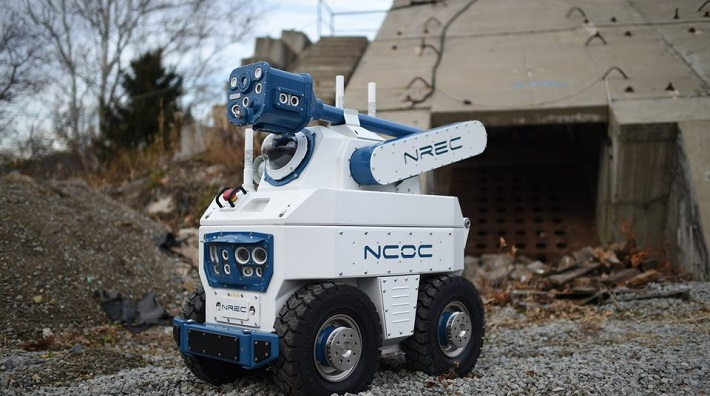
\includegraphics[width=0.95\textwidth]{figuras/sensabot.jpg}
		\caption{SENSABOT}
		\fonte{\citeonline{tractica2019sensabot}.}
		\label{fig:sensabot}
	\end{subfigure}%
	\begin{subfigure}{.5\textwidth}
		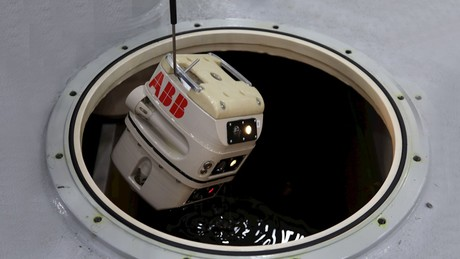
\includegraphics[width=0.95\textwidth]{figuras/abb.jpg}
		\caption{ABB}
		\fonte{\citeonline{processonline2019abb}.}
		\label{fig:abb}
	\end{subfigure}
	\caption{Robôs de inspeção}
\end{figure}

Independente de um robô ser controlado diretamente por uma pessoa, ou operar em modo completamente autônomo, em algum momento, a observação, supervisão e o julgamento humano ainda é um elemento crítico da atividade robótica.\par

A maior ligação perceptual entre um ambiente remoto e o operador de um robô, acontece através do vídeo enviado por uma (ou mais) câmera montada no robô. Existe uma relação forte entre problemas de localização da câmera e sua montagem, bem como angulo de visão e outros fatores que podem degradar essa ligação e deixar o operador vulnerável a uma serie de erros como: desorientação, falha ao reconhecer danos ou simplesmente não notar um ponto importante durante uma inspeção.\par

Estudos sugerem que disponibilizar uma câmera controlada independentemente da orientação de um robô, pode facilitar tarefas de localização num ambiente. \citeonline{hughes2004robotic}

A dificuldade de operação de um robô é proporcional ao seu grau de liberdade (DOF em inglês), isto é, quanto maior a variedade de movimentos o robô pode executar (considerando seu deslocamento, movimento de braços mecânicos e câmera), mais difícil é o controle para o operador.
Pensando nisso, o desenvolvimento de controles mais intuitivos para a câmera do robô diminui a complexidade geral do controle de movimentos totais do robô. \par

Com o objetivo de aprofundar os conhecimentos adquiridos ao longo do curso, este trabalho visa criar um controle de câmera do tipo (Pan e Tilt), baseando-se nos dados de movimento coletados e enviados de um smartfone, através de rede sem fio, acoplado a cabeça do operador. O projeto foi elaborado usando um Raspberry Pi, como unidade de controle dos servo motores da câmera e um celular smartfone Android, responsável por coletar e enviar informações referentes a posição espacial do aparelho. O desenvolvimento do projeto proporcionou um melhor entendimento em aspetos relacionados a rede de computadores, sistemas operacionais, interfaces de hardware, modulação por largura de pulso e desenvolvimento de sistemas para plataformas móveis.\par

Competências ligadas a construção de software puderam ser evoluídas, já que o módulo de controle , embarcado no Raspberry Pi, foi construído em linguagem C (usando bibliotecas de baixo nível para ativar sinais de PWM) e o módulo de coleta de dados foi desenvolvido em Java, usando a API do sistema operacional Android.

\begin{comment}
Alguns programas podem ser utilizados para auxílio da escrita do TCC entre eles o \textit{MathType} (com relação a equações), \textit{Inkscape} (com relação a imagens). \\ %enter

\textbf{PRIMEIRAS ORIENTAÇÕES}\\ %\textbf - negrito

1) O comando ``$\backslash$autoref\{label\}'' auto referencia o respectivo ``\textit{label}".

Exemplo 1: De acordo com o exposto no \autoref{chap:introducao}... Pode-se verificar na \autoref{fig:consumomundialporfonte-fig1}...\\

2) O comando ``$\backslash$citeonline\{bibid\}'' é utilizado para citações diretas. Ele cita o respectivo ``\textit{bibid}".\\

Exemplo 2:  Conforme \citeonline{AMARANTEMESQUITA20141261} cita em seu artigo, turbinas hidrocinéticas atualmente têm... \citeonline{VAZ2018509} também ressalta que turbinas de eixo horizontal possuem maiores...\\

\citeonline{vallverdu2014}  --->  Vallverdú (2014) --- DIRETA

\cite{vallverdu2014}   --->  (VALLVERDÚ, 2014) --- INDIRETA\\

O comando ``$\backslash$cite\{bibid\}'' é utilizado para citações indiretas. Ele cita o respectivo ``\textit{bibid}".\\

Exemplo 3: A máxima eficiência que uma turbina hidrocinética ideal pode alcançar é dada pelo Limite de Betz-Joukowski que corresponde a 59,3\%, o equivalente a um $C_P$ de 0,593 \cite{vallverdu2014, SHINOMIYA2015d}.\\ %Ao colocar a virgula, pode-se adicionar mais de um autor à citação.

3) Um ponto final é representado por um espaço entre os parágrafos.

Exemplo 1.
Exemplo 2.

Exemplo 3.

Exemplo 4.\\

4) Figuras

Figuras com extensão .jpg, .pdf, .eps, .ps, .png

As figuras devem ser adicionadas a pasta ``$\backslash$figuras'' no diretório deste template.

%[!htb] - são as opções onde o LaTeX escolhe a melhor posição para inserir a figura na página, aqui (here), topo (top) ou embaixo (bottom), respectivamente. Se você colocar apenas um deles, por exemplo [!h], a figura ficará exatamente onde você inseriu.

%Modelo de inclusão de figura. É só copiar, tomar como modelo e modificar.
\begin{figure}[H]
	\centering
	\caption{Consumo mundial de energia por fonte de energia em quatrilhões de BTU.}
	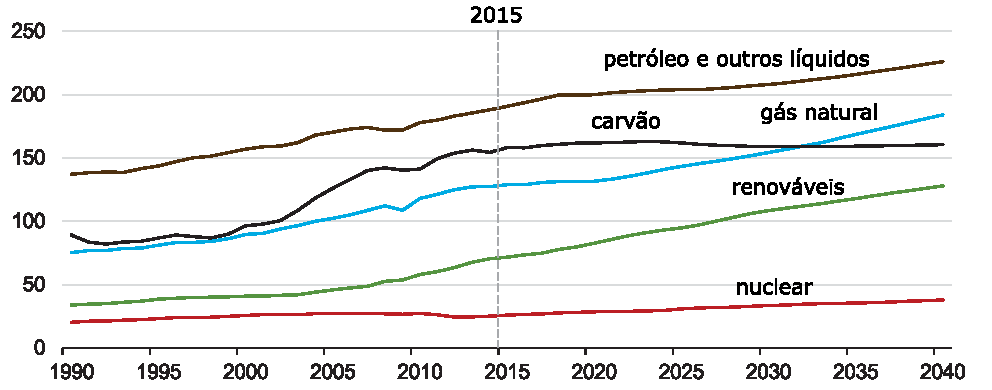
\includegraphics[width=1.0\textwidth]{figuras/consumodeenergiamundialporfonte.pdf}
	\fonte{\citeonline{harris2006essential}.}
	\label{fig:consumomundialporfonte-fig1}
\end{figure}

5) Referências

As referências devem ser adicionadas no arquivo ``base-referencias.bib'' no diretório deste template. 

Modelos podem ser editados na página ``https://truben.no/latex/bibtex/''. A partir do DOI pode-se encontrar o arquivo \textit{.bib} em ``https://www.doi2bib.org/''. No Google Acadêmico também se encontram bastantes referências no formato \textit{.bib}.

Tome cuidado com autores com nomes que termiam em Júnior, Filho, Neto e etc. Forma correta: ``Fulano Deltrano Siclano\{ \}Neto''.

As referências não reconhecem legal os pacotes de acentos. Então deve-se utilizar comandos de acentos. ``http://latexbr.blogspot.com/2011/02/acentos-e-caracteres-especiais.html''.

*Ao ser executado pela primeira vez, possa ser que você precise está conectado a internet para o programa instalar os \textit{packages} necessários para compilar o arquivo PDF.

Utilize esse \textit{template} sempre verificando as normas da Biblioteca Central da UFPA segundo o Guia para Elaboração de Trabalhos Acadêmicos disponível em http://bc.ufpa.br/ além das normas da ABNT.

Outras orientações podem ser encontradas na internet.\\

Boa escrita!

\section{Objetivos}
\label{sec:objetivos}

\subsection{Objetivo geral}
\label{subsec:objetivogeral}

Escreva seu objetivo geral aqui.

\subsection{Objetivos específicos}
\label{subsec:objetivosespecificos}

\begin{itemize}
\item Escreva seu objetivo específico 1 aqui;
\item Escreva seu objetivo específico 2 aqui;
\item ...;
\end{itemize}

\section{Estrutura do trabalho}
\label{sec:estrututaTrabalho}

Este trabalho está dividido em cinco seções, referências, anexos e apêndices.

Na seção 1 é apresentado o contexto no qual o trabalho está inserido, a justificativa e os objetivos almejados...

A revisão bibliográfica sobre as temáticas relacionadas com essa pesquisa é apresentada na seção 2...

A seção 3 mostra conceitos teóricos relacionados às ferramentas utilizadas no estudo tal como...

Na seção 4, os resultados são apresentados juntamente com suas devidas discussões, verificando...

Finalizando, a seção 5 faz as devidas conclusões e apresenta sugestões para trabalhos futuros.
\end{comment}